% !TEX encoding = UTF-8 Unicode
\documentclass[a4paper]{article}

\usepackage{color}
\usepackage{url}
\usepackage[T2A]{fontenc} % enable Cyrillic fonts
\usepackage[utf8]{inputenc} % make weird characters work
\usepackage{graphicx}

\usepackage[english,serbian]{babel}
%\usepackage[english,serbianc]{babel} %ukljuciti babel sa ovim opcijama, umesto gornjim, ukoliko se koristi cirilica

\usepackage[unicode]{hyperref}
\hypersetup{colorlinks,citecolor=green,filecolor=green,linkcolor=blue,urlcolor=blue}

\usepackage{listings}

%\newtheorem{primer}{Пример}[section] %ćirilični primer
\newtheorem{primer}{Primer}[section]

\definecolor{mygreen}{rgb}{0,0.6,0}
\definecolor{mygray}{rgb}{0.5,0.5,0.5}
\definecolor{mymauve}{rgb}{0.58,0,0.82}

\lstset{ 
  backgroundcolor=\color{white},   % choose the background color; you must add \usepackage{color} or \usepackage{xcolor}; should come as last argument
  basicstyle=\scriptsize\ttfamily,        % the size of the fonts that are used for the code
  breakatwhitespace=false,         % sets if automatic breaks should only happen at whitespace
  breaklines=true,                 % sets automatic line breaking
  captionpos=b,                    % sets the caption-position to bottom
  commentstyle=\color{mygreen},    % comment style
  deletekeywords={...},            % if you want to delete keywords from the given language
  escapeinside={\%*}{*)},          % if you want to add LaTeX within your code
  extendedchars=true,              % lets you use non-ASCII characters; for 8-bits encodings only, does not work with UTF-8
  firstnumber=1000,                % start line enumeration with line 1000
  frame=single,	                   % adds a frame around the code
  keepspaces=true,                 % keeps spaces in text, useful for keeping indentation of code (possibly needs columns=flexible)
  keywordstyle=\color{blue},       % keyword style
  language=Python,                 % the language of the code
  morekeywords={*,...},            % if you want to add more keywords to the set
  numbers=left,                    % where to put the line-numbers; possible values are (none, left, right)
  numbersep=5pt,                   % how far the line-numbers are from the code
  numberstyle=\tiny\color{mygray}, % the style that is used for the line-numbers
  rulecolor=\color{black},         % if not set, the frame-color may be changed on line-breaks within not-black text (e.g. comments (green here))
  showspaces=false,                % show spaces everywhere adding particular underscores; it overrides 'showstringspaces'
  showstringspaces=false,          % underline spaces within strings only
  showtabs=false,                  % show tabs within strings adding particular underscores
  stepnumber=2,                    % the step between two line-numbers. If it's 1, each line will be numbered
  stringstyle=\color{mymauve},     % string literal style
  tabsize=2,	                   % sets default tabsize to 2 spaces
  title=\lstname                   % show the filename of files included with \lstinputlisting; also try caption instead of title
}

\begin{document}

\title{Idealne studije\\ \small{Seminarski rad u okviru kursa\\Metodologija stručnog i naučnog rada\\ Matematički fakultet}}

\author{Bojan Veličković, David Živković, Marko Radosavljević, Darko Mladenovski\\ dzivkovicd1@gmail.com, bojanvelickovic76@gmail.com, 01marko.radosavljevic@gmail.com, darkomladenovski0@gmail.com}

%\date{9.~april 2015.}

\maketitle

\abstract{


\tableofcontents

\newpage

\section{Uvod}


\section{Osnovna uputstva}

\section{Engleski termini i citiranje}	

\section{Slike i tabele}

\section{K\^{o}d i paket listings}

\section{Prvi naslov}
\label{sec:naslov1}


\subsection{Uticaj organizacije fakulteta i kurseva na kvalitet studija}
\label{subsec:podnaslov1}

U okviru ankete, koju su ispitanici bili zamoljeni da urade, postavljena su pitanja o tome da li oni smatraju da je organizacija fakulteta bitna za idealne studije i da ocene
organizaciju na Matematičkom fakultetu. Preko 70\% ispitanika (njih 52) se izjasnilo da se u potpunosti slažu sa stavom da je organizacija bitna za idealne studije.\\
\begin{figure}[h!]
\begin{center}
    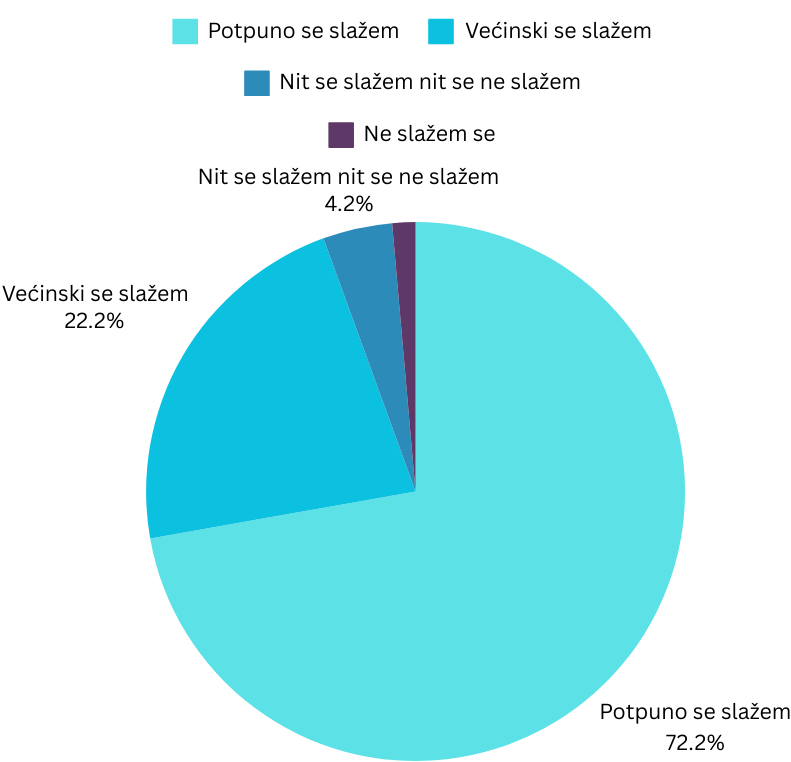
\includegraphics[scale = 0.3]{PieChartOrganizacija.png}
    \caption{Stavovi studenata o tome koliko je organizacija fakulteta bitna za kvalitet studija}
    \label{fig:organizacija}
\end{center}
\end{figure}
\\Takođe, većina studenata smatra da je za kvalitet studija bitno da imaju uticaj na to kako se kursevi polažu. Opcija da studenti biraju da li će imati predispitne obaveze ili projekte im u velikoj meri utiče na odluku da li su studije dobre ili ne.\\
\begin{figure}[h!]
\begin{center}
    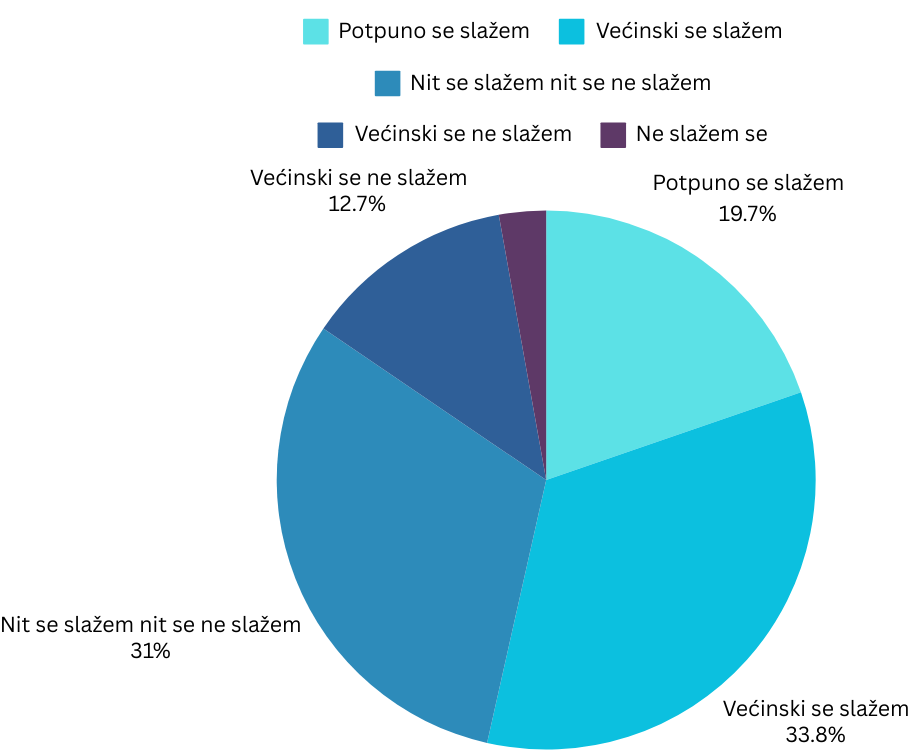
\includegraphics[scale = 0.3]{PieChartUticajNaPolaganje.png}
    \caption{Stavovi sudenata o tome koliko je bitno da imaju uticaj na to kako se ispiti polažu}
    \label{fig:uticaj}
\end{center}
\end{figure}\\
Kada smo tražili od ispitanika da ocene organizaciju na Matematičkom fakultetu, većina studenata nije bilo zadovoljno. 76\% ispitanika je dalo ocenu 1 ili ocenu 2, a 0 ispitanika je dalo ocenu 5. Glavni razlog za ovakve odgovore je bio manjak rokova za polaganje ispita, blisko praćen činjenicom da su teorija i praktični ispit najčešće u razdvojenim terminima, ali jako zavisni jedno od drugog.\\
\begin{figure}[h!]
\begin{center}
    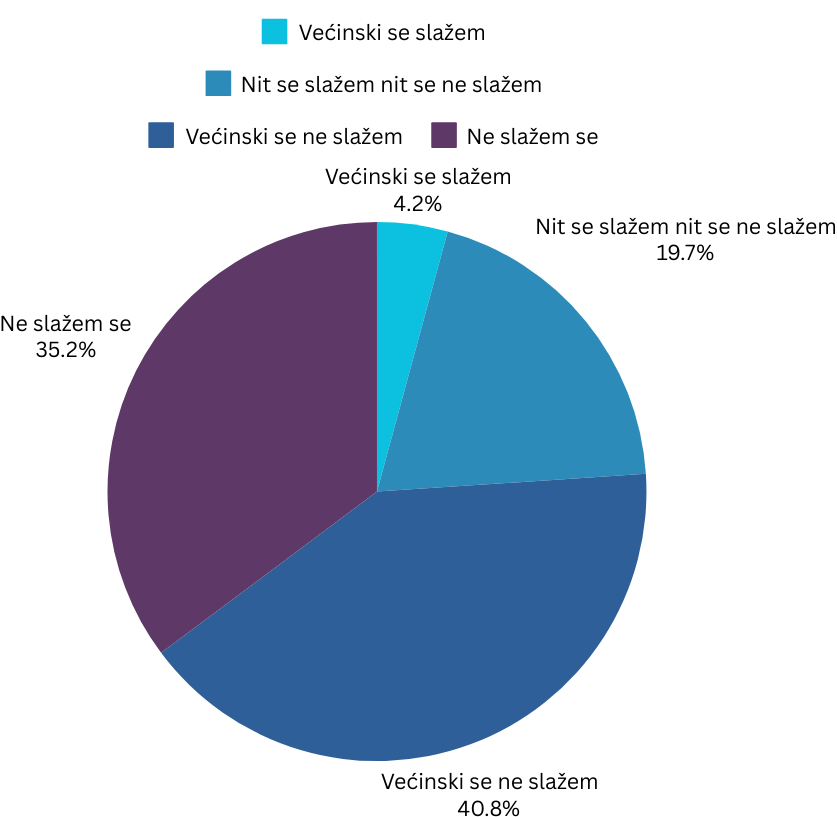
\includegraphics[scale = 0.3]{PieChartOrganizacijaMatf.png}
    \caption{Ocene organizacije na Matematičkom fakultetu}
    \label{fig:organizacija_matf}
\end{center}
\end{figure}


\subsection{Uticaj povratnih informacija o napretku studenata na kvalitet studija}
\label{subsec:podnaslov2}

Povratne informacije o napretku u velikoj meri utiču na samopouzdanje studenata, a studenti koji su sigurni u sebe i svoje znanje nakon studija će za uzvrat oceniti svoj fakultet bolje. Većina ispitanika smatra da je za idealne studije neophodno da u toku studija često dobijaju povratne informacije kako bi se osećali sigurnije. \\
\begin{figure}[h!]
\begin{center}
    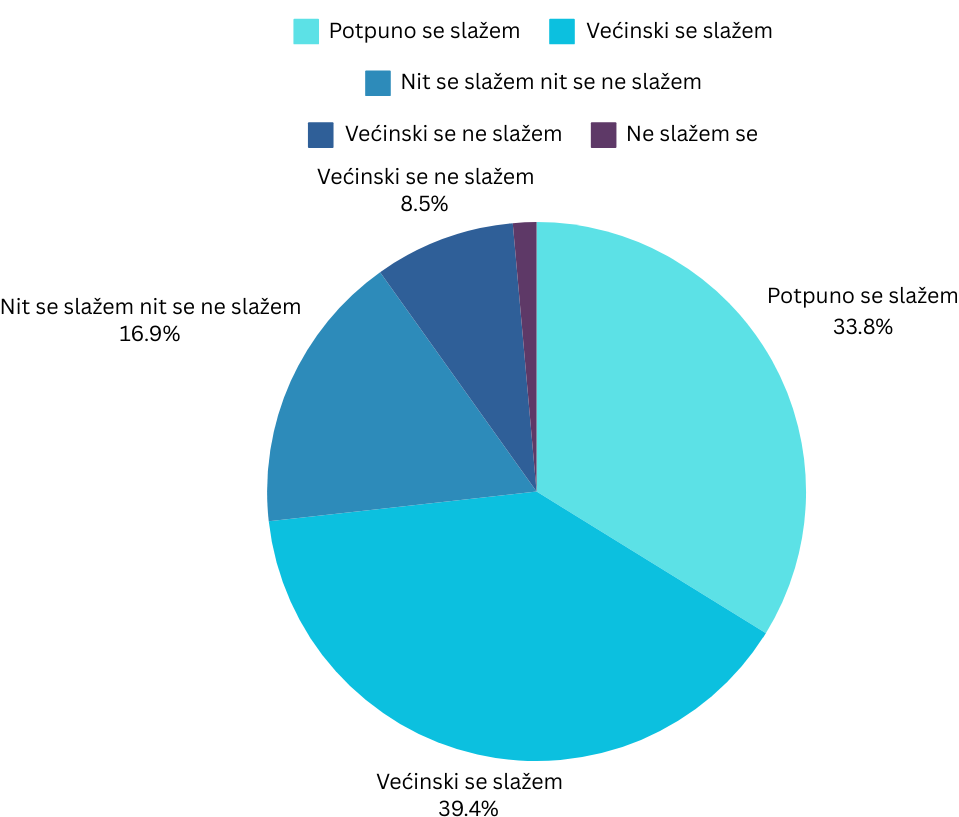
\includegraphics[scale = 0.3]{PieChartPovratneInformacije.png}
    \caption{Stavovi o važnosti povratnih informacije u toku studija}
    \label{fig:povratne_informacije}
\end{center}
\end{figure}
\\Na Matematičkom fakultetu, studenti se većinski slažu da skoro nikada nisu dobijali povratne informacije o svom napretku tokom studija. 67.6\% (48) studenata su rekli da su jako retko ili da nikada nisu dobijali ovu vrstu potvrde napretka. Ova činjenica ima uticaj na samopouzdanje studenata, pa su iz tog razloga ove vrste potvrda neophodne za idealne studije. \\
\begin{figure}[h!]
\begin{center}
    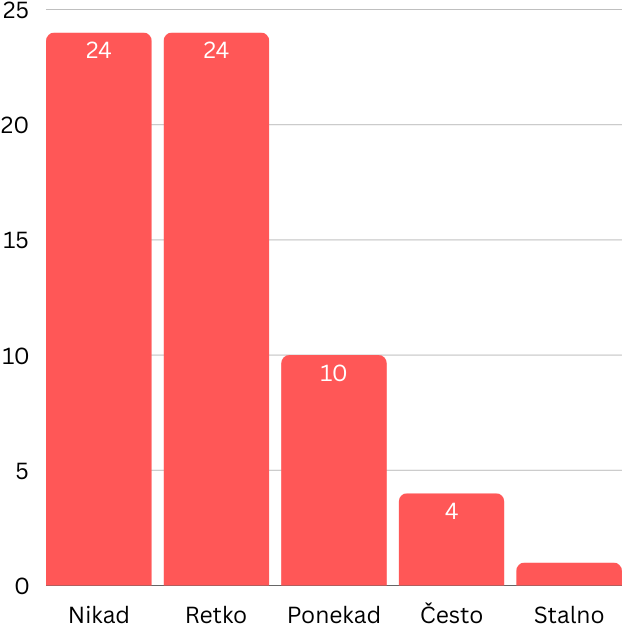
\includegraphics[scale = 0.3]{PovratneInformacijeMatf.png}
    \caption{Učestalost povratnih informacija o napretku na Matematičkom fakultetu}
    \label{fig:povratne_informacije_matf}
\end{center}
\end{figure}
\\Većina studenata Matematičkog fakulteta (njih 32) je donekle siguran u svoje znanje. Potpuno sigurnih studenata (njih 9) ima isto koliko i onih koji nisu uopšte sigurni (njih 1) ili su većinski nesigurni (njih 8).\\
\begin{figure}[h!]
\begin{center}
    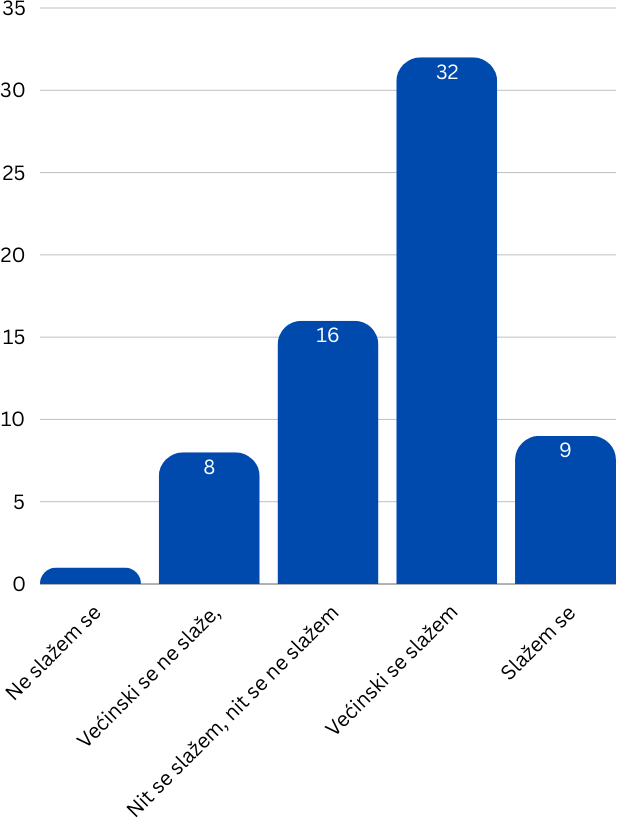
\includegraphics[scale = 0.3]{SamouverenostStudenataMatf.png}
    \caption{Koliko su studenti Matematičkog fakulteta samouvereni u svoje znanje}
    \label{fig:samouverenost_matf}
\end{center}
\end{figure}
\\
Takođe, postoji velika količina literature na temu uticaja samouverenosti studenata u svoje znanje na njihov proces učenja. Profesori i mentori imaju veliki uticaj na samopouzdanje svojih ucenika, a to loše samopouzdanje često negativno utiče na napredak studenta \cite{G1}. 
Samopouzdanje studenata je podatak na osnovu kog se može jako dobro predvideti njegov napredak.\cite{G2}



\section{n-ti naslov}

\section{Zaključak}


\renewcommand{\refname}{Literatura}
\begin{thebibliography}{9}

\bibitem {G1} \href{https://www.researchgate.net/publication/341003040_Students'_Self-Confidence_and_Its_Impacts_on_Their_Learning_Process}{Students’ Self-Confidence and Its Impacts on Their Learning Process}

\bibitem {G2} \href{https://pmc.ncbi.nlm.nih.gov/articles/PMC4278496/}{Correlating Student Knowledge and Confidence Using a Graded Knowledge Survey to Assess Student Learning in a General Microbiology Classroom}

\end{thebibliography}


\end{document}
